\documentclass[a4paper,12pt]{article}
\usepackage[italian]{babel}
\usepackage[utf8]{inputenc}
\usepackage{graphicx} %per aggiungere le immagini
\usepackage{listings} %per aggiungere codice sorgente

\newenvironment{cypher}{\begin{lstlisting}[keepspaces=true]}{\end{lstlisting}}

\pagenumbering{arabic}
\linespread{1.25}
\begin{document}

\section*{L'algoritmo PageRank}
PageRank è un algoritmo introdotto da Google per classificare le pagine web. 
Nasce dalla necessità del motore di ricerca di avere un ordinamento delle 
pagine web rispetto alla loro importanza. A detta di Google, esso funziona 
contando il numero di link delle pagine web per avere una stima approssimativa 
della qualità e dell'importanza di un sito web. L'assunzione su cui questo si 
basa è quella che, tantopiù una pagina è importante, più tende a ricevere 
collegamenti dalle altre pagine.
\begin{figure}[h!]
  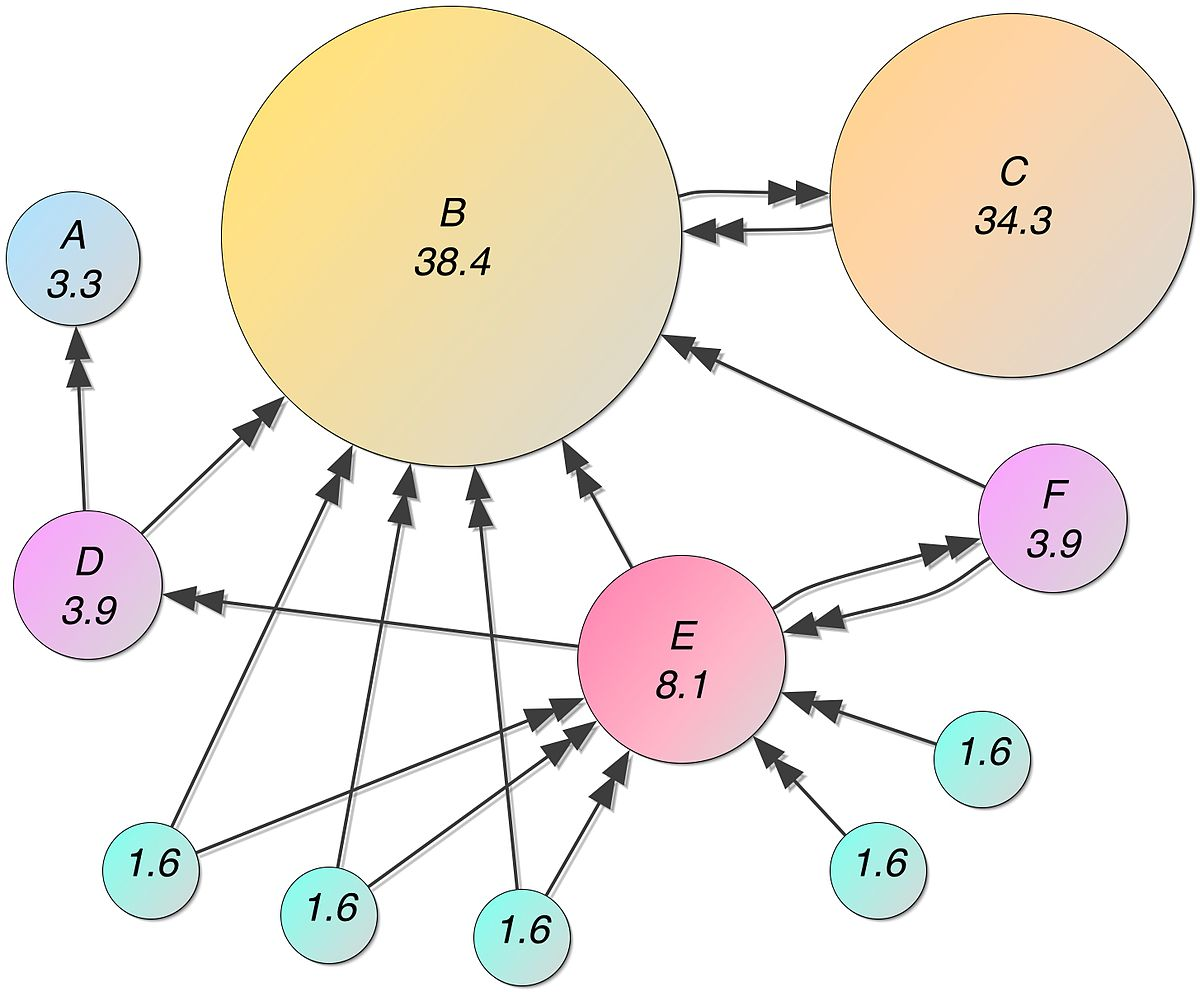
\includegraphics[width=\linewidth]{images/pagerank.jpg}
  \caption{Rappresentazione grafica del ranking con PageRank}
\end{figure}

\section*{Basi di dati a grafo}
Per l'elaborazione dei dati relativi alle varie relazioni tra autori e articoli 
accademici, si è visto naturale l'utilizzo di una base di dati a grafo. \\
Questo particolare tipo di base di dati offre le ottimizzazioni necessarie a 
rappresentare un enorme numero di relazioni tra entità, in modo dinamico, 
senza dover racchiudere lo schema in convenzionali tabelle. Offre, altresì, 
convenienti operazioni e algoritmi pre-implementati per l'analisi e 
l'elaborazione dei grafi.
\par
La principale caratteristica che differenzia le basi di dati di grafi rispetto 
alle classiche basi di dati relazionali è che le operazioni di join, mentre 
nel modello relazionale sono svolte a tempo di interrogazione, facendo il 
matching delle chiavi primarie e delle chiavi esterne di tutte le righe della 
nelle tabelle interrogate, operazione tra l'altro pesante sia dal punto di 
vista computazionale che dell'utilizzo di memoria, sono ottimizzate conservando 
le relazioni all'interno dei nodi stessi. Viene sacrificata, così, la 
dimensione su disco del database, a vantaggio di una ridotta complessità delle 
operazioni di join.
\section*{Il Graph DBMS Neo4J}
Tra le opzioni presenti, la scelta è ricaduta su Neo4J, il dbms di grafi più 
diffuso sulla piattaforma Java. Esso possiede due diverse distribuzioni: 
neo4j-community e neo4j-enterprise. La distribuzione enterprise è pensata per 
l'utilizzo in cloud, offrendo soluzioni con un maggiore parallelismo per 
l'esecuzione degli algoritmi, la possibilità di eseguire algoritmi su cluster, 
e, a dire degli autori, un runtime per l'esecuzione delle query in linguaggio 
Cypher del 70\% più veloce. \\
Non essendoci la necessità di esecuzione in cloud si è scelto di utilizzare 
la distribuzione community. \\
Neo4J introduce un suo linguaggio di querying per l'interazione dell'utente con 
il database. Tale linguaggio nasce con l'obiettivo di essere facilmente 
leggibile e comprensibile dagli utenti, fornendo, allo stesso tempo, le 
features necessarie a gestire convenientemente i grafi, a differenza del 
classico linguaggio SQL.
Di seguito si fornisce una breve panoramica delle possibilità del linguaggio 
Cypher.
I nodi del grafo sono rappresentati, nelle query Cypher, da un nome racchiuso 
tra due parentesi tonde (che rappresentano la circonferenza con cui si suole 
rappresentare i nodi nelle rappresentazioni grafiche dei grafi). La ricerca nel 
database si effettua attraverso l'istruzione MATCH seguita dall'oggetto da 
cercare.
MATCH (a) seleziona tutti i nodi del grafo, che vengono rappresentati nella 
query dal nome "a". Sono selezionati tutti i nodi del grafo perché non sono 
presenti vincoli.
MATCH (a: Author) seleziona, invece, i nodi che hanno come tipo Author. I tipi 
non vanno dichiarati precedentemente all'uso, ma lo schema è generato 
dinamicamente. Il tipo Author farà parte del database quando sarà creato il 
primo nodo di tale tipo.
E' possibile filtrare ulteriormente utilizzando vincoli sui campi che possiede 
un dato nodo:
MATCH (a: Author {name: "Giuseppe Rossi"}) seleziona tutti i nodi di tipo 
Author per cui esista un campo denominato "name" il cui valore sia la stringa 
"Giuseppe Rossi". Data l'assenza di una fase separata per la definizione dello 
schema della base di dati, nulla vieta di avere nodi di tipi diversi che 
abbiano campi con nomi e tipi diversi. Tuttavia, questa diversificazione può 
essere deleteria ad una buona gestione di una base di dati. A tal proposito
Neo4j permette la definizione di vincoli che permettano, oltre che a mantenere
dati i coerenti, a rendere efficienti le interrogazioni attraverso l'utilizzo
di indici.
Un vincolo utile per l'ottimizzazione delle query è quello di unicità. E'
possibile aggiungere il vincolo di unicità attraverso una query Cypher:
\begin{lstlisting}[keepspaces=true]
  CREATE CONSTRAINT ON (book:Book)
    ASSERT book.isbn IS UNIQUE
\end{lstlisting}
Attraverso questo comando si può istruire il database che la il campo denominato
isbn dei nodi di tipo Book è unico. Per unico si intende che in tutta la base di
dati non esistono due nodi distinti di tipo Book con lo stesso isbn. Essendo
presente questo vincolo, la base di dati procede all'indicizzazione del campo
isbn. In tal modo le query successive di MATCH sul campo isbn avranno la stessa
velocità di quelle effettuate sull'ID del nodo.
\par
La creazione dei nodi avviene attraverso la parola chiave CREATE. Attraverso la
parola chiave CREATE è possibile aggiungere sia nodi che relazioni alla base di
dati. \\
Per creare un nodo si usa una sintassi simile a quella usata per MATCH:
\begin{lstlisting}[keepspaces=true]
  CREATE (a: Author {name: "Giuseppe Rossi"})
\end{lstlisting}
Per creare, invece, una relazione tra due nodi esistenti, si utilizza la seguente
sintassi:
\begin{lstlisting}[keepspaces=true]
  MATCH (a: Author {name: "Giuseppe Rossi"}),
    (b: Author {name: "Francesco Bianchi"})
  CREATE (a)-[:COAUTHOR]->(b)
\end{lstlisting}
In tal modo si definisce un arco orientato dal nodo a al nodo b. \\
Anche le relazioni possono avere, come i nodi, dei campi. Questi si definiscono
utilizzando una sintassi simile a quella utilizzata per definire campi nei nodi:
\begin{lstlisting}[keepspaces=true]
  MATCH (a: Author {name: "Giuseppe Rossi"}),
    (b: Author {name: "Francesco Bianchi"})
  CREATE (a)-[:COAUTHOR {times: 1}]->(b)
\end{lstlisting}
Per poter inserire qualcosa che si avvicini alla nozione di pesi di un arco, è
utile poter inserire un contatore numerico, aggiornandolo ad ogni nuovo matching.
Per questo scopo esiste una seconda parola chiave del linguaggio Cypher che
equivale a fare match su un nodo o su una relazione; se il matching esiste allora
si esegue una sotto-query relativa al matching, se non esiste si esegua un'altra
sotto-query relativa alla creazione.
\begin{lstlisting}[keepspaces=true]
  MATCH (a: Author {name: "Giuseppe Rossi"}),
        (b: Author {name: "Francesco Bianchi"})
  MERGE (a)-[c:COAUTHOR]->(b)
  ON CREATE SET c.times = 1
  ON MATCH SET  c.times = c.times + 1
\end{lstlisting}
\end{document}
